\subsection{Networking}
\label{sub:networking}
Networking in MicroNet has been discussed in detail in section 6.5 Networking
Implementation in project thesis one \cite{biedermann2015project1}. The original
implementation was improved in the course of all three theses and this section
provides a summary of the final implementation solution of networking.

Networking is the most fundamental aspect of an \og{} development and crucial
for the stability of \ms{} applications. The networking concept for \ms{}
applications is heavily influenced by the IDEAL tenet because it makes it
necessary to provide an abstract messaging concept that is decoupled from any
implementation.

In MicroNet this network abstraction is realized by defining a set of networking
capabilities that must be supported by the underlying network technology. These
capabilities are represented in the form of the \code{IPeer} Java interface
shown in \autoref{lst:ipeer_interface}. Standard services can therefore
communicate over an instantiation of the \code{IPeer} interface injected by the
framework. This makes the underlying technology exchangeable since the interface
is stable. This allows platform independence as long as the services are written
in Java.

\begin{figure}
	\begin{lstlisting}[language=Java,firstnumber=1] 
public interface IPeer {
	void startup(URI host);
	void shutdown();
	
	void sendRequest(URI destination, Request request);
	void sendRequest(URI destination, Request request, 
		Consumer<Response> handler);
		
	Response sendRequestBlocking(URI destination, Request request);
	Response sendRequestBlocking(URI destination, Request request,
		int timeout);
		
	void listen(String path, Consumer<Request> handler);
	void listen(String path, Function<Request, Response> handler);
}
	\end{lstlisting}
  	\caption{The iPeer interface must be implemented to participate in MicroNet
  	applications.}
  	\label{lst:ipeer_interface}
\end{figure}

MicroNet implements this networking interface by relying on ActiveMQ as a
message broker. Although it would be possible to replace ActiveMQ as the
MicroNet networking technology this is out of the scope of this thesis to be
validated in practice. As a result MicroNet is heavily dependent on ActiveMQ.

According to the polyglot programming tenet it is a requirement that arbitrary
technologies can participate in a \ms{} application despite the tight coupling
with ActiveMQ. To accomplish this an adapter must be implemented to couple the
foreign technology with the application. The adapter can be an
implementation of an equivalent messaging interface in another programming
language using one of the many proposed ways to integrate with ActiveMQ like
RESTful HTTP, JMS, .NET, C/C++, Go, Node.js, Python, and more.

For game engine integration the messaging interface also has to be implemented
in the respective technology of the engine. In the case of MicroNet ActiveMQ
Unity3D is used as the refernce game engine which is written in C\#. For this
purpose the NMS \gls{api} which is a .NET port of the Java Message Service (JMS)
interface is used to make MicroNet accessible from the Unity3D game engine.

\subsubsection{Messaging System}

Messaging in MicroNet evolves around patterns: API Gateway, Reverse Proxy and
Pipes and Filters.

MicroNet uses a reverse proxy to interchange messages from the public Internet
with the internal network used by MicroNet. For this purpose two separate
message brokers are used and only the public broker is exposed to the Internet.
The gateway intercepts all messages from the public network and forwards them to
the responsible \ms{}. This is further detailed in the \textit{Messaging API}
section below.

The reverse proxy in fact also is the API gateway. An API gateway is a standard
approach offering the \textit{Service API} to the users. Upon reception of a
message the gateway can filter it according to a white- or blacklisting approach.

\begin{figure}
\begin{lstlisting}[language=Java,firstnumber=1] 
@MessageService(uri = "mn://foo")
public class ServiceFoo {
	@OnStart
	public void onStart(Context context) {
		URI destination = URI.create("mn://bar/hello");
		Request request = new Request("Hello from Foo!");
		context.getPeer().sendRequest(destination, request, response -> {
			System.out.println("Received Response: " + response.getData());
		});
	}
}

@MessageService(uri = "mn://bar")
public class ServiceBar {
	@MessageListener(uri="/hello")
	public Response helloHandler(Context context, Request request) {
		System.out.println("Received Request: " + request.getData());
		return new Response(StatusCode.OK, "Likewise, Bar");
	}
}
\end{lstlisting}
\caption{Two MicroNet services communicating with each other.}
\label{lst:service_communication}
\end{figure}

\mss{} can access the messaging functionality by using the context object
injected by the framework. \autoref{lst:service_communication} shows an example
of two simple \mss{} communicating with each other. It has to be mentioned that
the two services in the listing are fully functional without any additional
code necessary. The setup of the context and the \ms{}'s main function are
completely abstracted by the framework.

\paragraph{Message Parameters}

One useful feature that MicroNet provides are typed message parameters. These
parameters are defined using Parameter Codes and the \textit{Template Types}
both defined int the \textit{Shared Model}.

Message parameters spare the developer the need to individually define a
specific payload for each message transfer. For example slightly different
messages can be distinguished by only using parameter codes and leaving the
payload unchanged.

\begin{figure}
\begin{lstlisting}[language=Java,firstnumber=1] 
@MessageService(uri = "mn://foo")
public class ServiceFoo {
	@OnStart
	public void onStart(Context context) {
		URI destination = URI.create("mn://bar/hello");
		Request request = new Request("Hello from Foo!");
		request.getParameters().set(ParameterCode.ID, 42);
		context.getPeer().sendRequest(destination, request);
	}
}

@MessageService(uri = "mn://bar")
public class ServiceBar {
	@MessageListener(uri="/hello")
	public void helloHandler(Context context, Request request) {
		int parameter = request.getParameters().getInt(ParameterCode.ID);
		System.out.println("Received Request with Parameter: " + parameter);
	}
}
\end{lstlisting}
\caption{Adding a parameter to a MicroNet message.}
\label{lst:message_parameters}
\end{figure}

\autoref{lst:message_parameters} shows how services can transmit parameters
along with a request. For responses this works exactly the same.

\subsubsection{Connection Authentication}

Security is always a concern in regard to Internet applications. The backbone
of distributed application security is user connection authentication.
Since multiple gateways can be active simultaneously the integrity of the user
has to be validated by the gateway with every request. The gateway validates the
user request by looking up the user connection in the session store and
comparing it to the connection the request was received from. If no user session
is present in the session store the user connection is considered
unauthenticated.

For unauthenticated connections the gateway only forwards login messages to the
login service. Upon a positive login response from the account service the
processing gateway adds the user connection to the session store. Other gateways
are then able to look up if a connection is authenticated. The advantage of this
solution is that it scales very well. The downside is that it involves many
reads of the session store.

A requirement for this approach to work is that the underlying networking
provides a way to correlate incoming messages with a connection. This can be
done generating a connection ID hash based upon the user's IP/port combination.
ActiveMQ has this capability already built in by providing a globally unique
connection ID per connection.

The connection authentication process is further explained in
\autoref{sub:session_management}.

\subsubsection{MicroNet Messaging API}

The \textit{Messaging API} provided by a MicroNet applications is a direct implementation
of the fine-grained interfaces tenet. It offers the following functionality to
promote stateless message transfers:

\begin{itemize}
  \item Sending a request to a \ms{} either from a user or another \ms{}
  \item Sending a request to a \ms{} and waiting for a response with a
  short\footnote{5 - 15 seconds of timeout seem appropriate for most short
  requests.} timeout either from a user or another \ms{}
  \item Sending an event to a user from a \ms{}
  \item Sending an event to a group of users from a \ms{}
  \item Sending a message to a topic, meaning to all subscribed \mss{}
  \item Named message parameters
\end{itemize}

\begin{figure}
	\centering
	\hspace*{-1.5cm}
	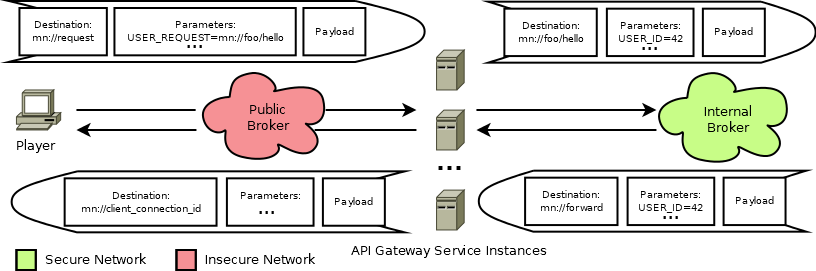
\includegraphics[width=1.2\textwidth]{images/architecture/MessagingAPI}
	\caption{The API Gateway offers the MicroNet \textit{Messaging API} to the player.}
	\label{fig:messaging_api}
\end{figure}

These messaging capabilities are sufficient to model any arbitrary message
transfer. They leave a great degree of freedom and make message transfer
implementation very comfortable. 

\autoref{fig:messaging_api} shows the communication between a user and a
MicroNet application. The user in this scenario is already authenticated so the
gateway only needs filter client quests according to access restrictions. The
user sends his request to the \code{mn://request} queue which leads to an
arbitrary gateway instance consuming the request. The gateway reads the
\code{USER\_REQUEST} parameter from the request and according to it forwards the
message to the internal broker. Depending on the situation if the user expects a
response within the defined timeout or if no response is expected the
gateway holds on to a temporary response queue which allows immediate responses.
Such an immediate response can also indicate that the request will need longer
to be processed and therefore the requestor has to act accordingly and wait for
an asynchronous response.

These asynchronous responses are called events. An event can either be sent to a
single user or to a group of users. For this purpose \mss{} can send a request
to the \code{mn://forward} queue which is consumed by any gateway who in
response forwards the event to the corresponding user or group.

One last feature of the MicroNet \textit{Messaging API} is the ability to send messages
to topics which can be subscribed by any service. This allows services to react
on events happening throughout the application. This can be for example the
\textit{new player connected} event.











